% begin module approximate integration
\begin{frame}
\frametitle{}
\begin{example}
Use Simpson's Rule with $n=4$ to approximate $\ds \int_0^4 (\frac18x^2+1)dx$.\\
{\bf{Solution:}}\\
\uncover<2->{%
\[
S_n= \frac{\Delta x}3\left[f(x_0)+4f(x_1)+2f(x_2)+4f(x_3)+\dots +f(x_n)\right]
\]
} %
\uncover<3->{%
Here, $ \Delta x = \frac{4}{n} = 1$
} %
\begin{columns}
\begin{column}{.7\textwidth}
\uncover<4->{%
\begin{align*}
S_4& =\frac{1}{3}[f(0)+4f(1)+2f(2)+4f(3)+f(4)]\\
   & =\frac13\left(1+4\cdot \frac94+2\cdot \frac32 +4\cdot \frac{17}{8} +3 \right) =\frac{20}{3} 
\end{align*}
}
\uncover<5->{%  
What is the exact value?
}
\uncover<6->{%
\[\int_0^4 (\frac{x^2}{8}+1) dx=\left[\frac{x^3}{24}+x\right]_0^4=\left(\frac83+4\right)-(0)=\frac{20}{3}
\]
}
\end{column}
\only<7>{\movie[autostart]{}{../../modules/approximate-integration/sweet.au}
}
\begin{column}{.25\textwidth}

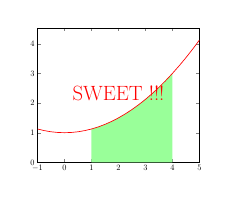
\begin{tikzpicture}[scale=.3]
  \begin{axis}[
    %grid=both,
    ymin=0,
    xmin=-1,xmax=5,
    %axis on top
    ]
    \addplot[draw=none,domain=1:4,fill=green!40] {x^2/8+1}\closedcycle;
    \addplot[solid,thick,red,domain=-1:5] {x^2/8+1};
  \only<7>{  \node[above,text=red, font=\Huge] at (axis cs:2,2) {SWEET !!!};
  } %
  \end{axis}
\end{tikzpicture}

%\begin{tikzpicture}
%  \node (img1) {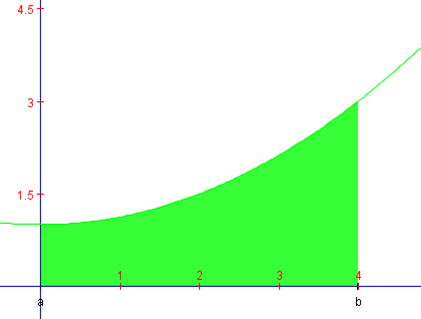
\includegraphics[width=\linewidth]{../../modules/approximate-integration/pictures/S5}};
%  \node (img2) at (img1.south west) [yshift=1cm, xshift=1.7cm] {\includegraphics<7>[width=.7\linewidth]{../../modules/approximate-integration/pictures/sweet}};
%\end{tikzpicture}

% 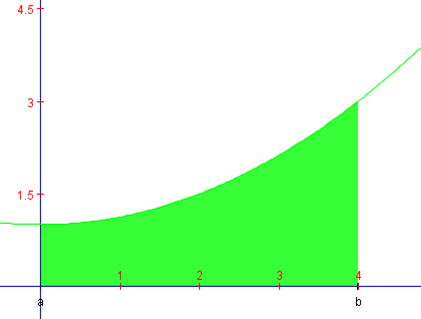
\includegraphics[width=\linewidth]{../../modules/approximate-integration/pictures/S5}
 %\includegraphics<7>[width=\linewidth]{../../modules/approximate-integration/pictures/S6}
\end{column}

\end{columns}

\end{example}

\end{frame}
% % % % % % % % % % % % % % % % % % % % % % % % % % % % % % % %

